\documentclass[10pt, a4paper]{article}
\usepackage{helvet}
\renewcommand{\familydefault}{\sfdefault}
\usepackage[english]{babel}
\usepackage[utf8x]{inputenc}
% package for including graphics with figure-environment
\usepackage{graphicx}
\usepackage{hyperref}
\usepackage{subcaption}
% colors for hyperlinks
% colored borders (false) colored text (true)
\hypersetup{colorlinks=true,citecolor=black,filecolor=black,linkcolor=black,urlcolor=black}

% package for bibliography
\usepackage[authoryear,round]{natbib}
% package for header
\usepackage[automark,headsepline]{scrlayer-scrpage}
\pagestyle{scrheadings}
\ihead[]{Text Detection in Natural Scene Images}
\ohead[]{September 30, 2021}
\cfoot[]{\pagemark} 

\begin{document}
	\title{
	\begin{figure}[!ht]
		% \flushleft
			
\includegraphics[width=0.26\textwidth]{img/htwlogo.jpg}
	\end{figure}
	\vspace{1cm}
	\Huge Text Detection in Natural Scene Images \\
	using CRAFT and EAST
	}
	
	\vspace{1cm}
	
	% if you are the only author, you might use the following
	% \author{Name of student}	
	
	% Insert here your name and correct mail address
	\author{\Large \href{mailto:s0566146@htw-berlin.de}{Henry Febrian}
	\vspace{1cm}}
	
	% name of the course and module
	\date{
	\large Module: \textit{Computergrafik und Bildverarbeitung} \\
	\vspace{0.8cm}
	\large Lecturer: Erik Rodner \\
	\vspace{1cm}
	\large September 30, 2021
	}

	\maketitle
	\setlength{\parindent}{0pt}

\vspace{2cm}
\begin{abstract}
To be edited at a later date. 

\end{abstract}
	\newpage
	\tableofcontents
	\newpage
	
\section{Introduction} % (fold)
\label{sec:introduction}
Text is arguably one of the most essential form of communication. According to \cite{LongEtAl}: 
\begin{quotation}
	\emph{``As the written form of human languages, text makes it feasible to reliably and effectively spread or acquire information across time and space. In this sense, text constitutes the cornerstone of human civilization.''} 
	\citep{LongEtAl} 
\end{quotation}
In the modern world, text as a medium of communication is not only consumed by humans but has claimed its place in the world of technology.
However, text detection in natural scene images is proven to be challenging. Compared to detecting text on handwritten materials, the randomness of a natural scene is a big hurdle to overcome.
This paper aims to test and evaluate the two proposed methods on their performance in detecting natural-scene texts. It begins by observing the interference found on natural scenes followed by introducing and giving an overview of CRAFT and EAST.
It then presents an overview on the how text is detected using the two methods, along with an explanation of the evaluation dataset. Subsequently, the performance review of the algorithm will be presented, which is obtained by testing the preferred method on the aforementioned dataset.
% section introduction (end)

\section{Challenges of Natural Text Detection} % (fold)
\label{sec:challenges}
Natural scene images could be classified as images which are taken in uncontrolled environments, with any device ranging from smartphones to professional cameras. These images are snapshots of things in the real world.
\begin{figure}[h!]
	\centering
	\begin{subfigure}[b]{0.4\linewidth}
	  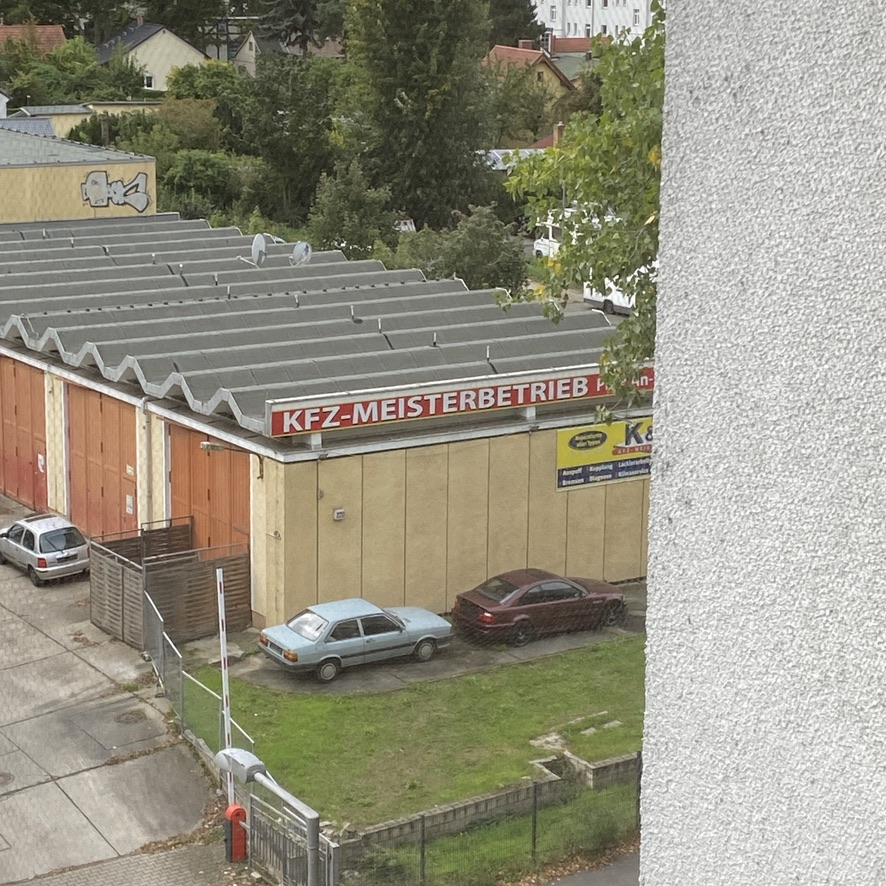
\includegraphics[width=\linewidth]{img/sample2.jpeg}
	  \caption{A scenery}
	\end{subfigure}
	\begin{subfigure}[b]{0.4\linewidth}
		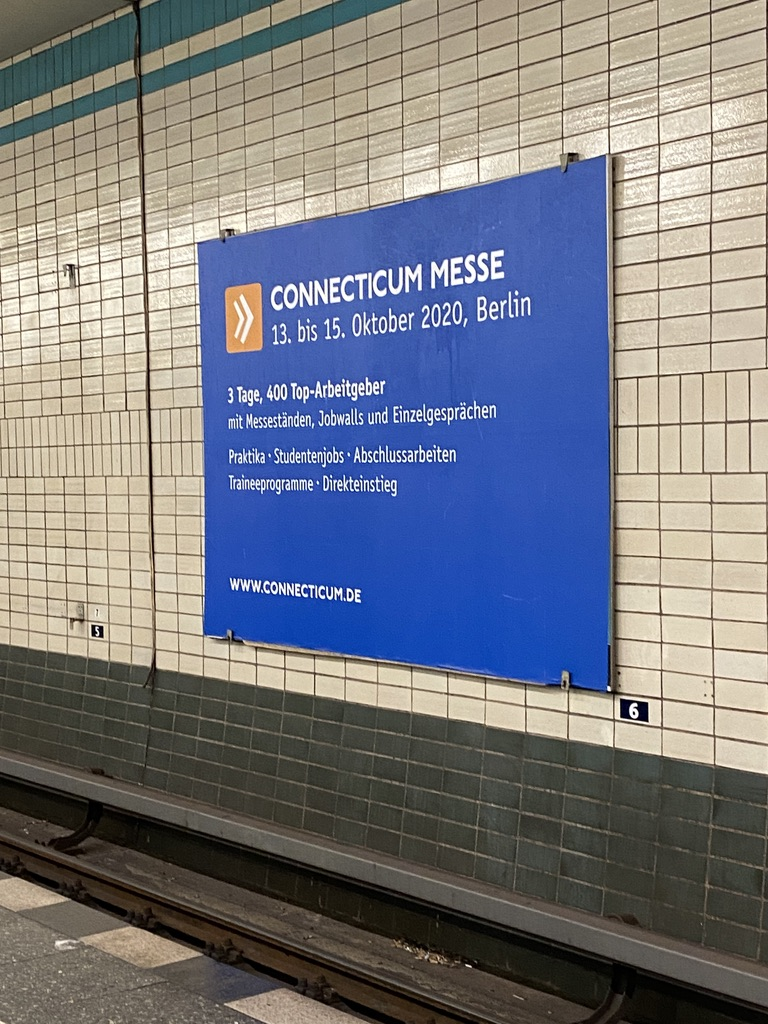
\includegraphics[width=\linewidth]{img/sample3.jpeg}
		\caption{A billboard}
	  \end{subfigure}
	\caption{Samples of natural scene images.}
	\label{fig:samples}
  \end{figure}

The random nature of the real world, combined with the diversity of available devices introduced some factors which make natural text detection a greater challenge than detecting structured text in documents. \cite{NaturalScene} mentioned some conditions that are found in natural scene which may significiantly impact text detection procedure. They are:
\begin{itemize}
	\item Raw sensor image and sensor noise
	\item Viewing angle
	\item Blur
	\item Lighting
	\item Resolution
	\item Non-paper objects
	\item Non-planar objects
\end{itemize}
Although devices have evolved to a point where most of handheld devices are capable of shooting in a high resolution, low-end handheld cameras and older models still struggle in this sector.
Uncontrolled environment, combined with the possible lack of stabilization from the equipment can cause blur \citep{Rosebrockeast}. Also, there are countless factors such as the time of the day, weather, camera flash, and many others which may impact the lighting conditions, further hindering the ability to detect text. Non-paper objects such as glass and plastic may reflect images, and non-planar objects such as text wrapped around a bottle becomes distorted and deformed \citep{Rosebrockeast}.
Additionally, there might be patterns that are extremely similar to text, or occlusions caused by foreign objects, which may potentially lead to confusion and mistakes \citep{LongEtAl}.
% section challenges (end)

\clearpage

\section{Overview of the Methods} % (fold)
\label{sec:overviewmethods}
\subsection{Overview of EAST} % (fold)
\label{sub:overvieweast}
According to \cite{EastZhouEtAl}, the key component of EAST is a neural network model, which is trained to directly predict the existence of text instances and their geometries from full images \citep{EastZhouEtAl}.
Hence, the abbreviation EAST: Efficient and Accurate Scene Text Detector.
\begin{figure}[hbt!]
	\centering
	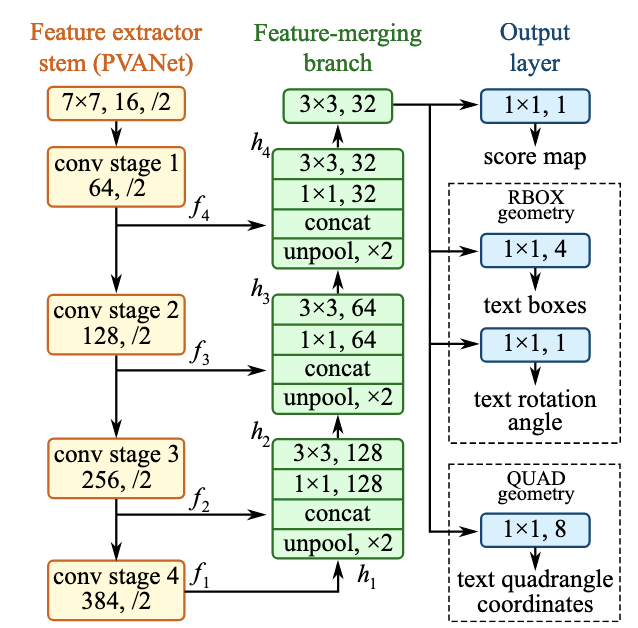
\includegraphics[width=0.5\textwidth]{img/eaststructure.png}
	\caption{Schematic view of EAST, adopted from Figure 3 of~\protect\cite{EastZhouEtAl}}
	\label{fig:east1}
\end{figure}

As claimed by \cite{EastZhouEtAl}, EAST is among the most efficient text detectors that achieve state-of-the-art performance on benchmarks.
The idea of the network is described shortly below:
\begin{quotation}
	\emph{``... we adopt the idea from U-shape \citep{unet}
	to merge feature maps gradually, while keeping the upsampling branches small. Together we end up with a network that can both utilize different levels of features and
	keep a small computation cost.''} 
	\citep{EastZhouEtAl} 
\end{quotation}
It is capable of predicting text on 720p images, running at an average of 13 FPS. The fastest setting, which reached a speed of 16.8 FPS was achieved on a combination of their algorithm with PVANET on 720p images using NVIDIA Titan X graphics card. \citep{EastZhouEtAl}.
The training of the network is further described as follow:
\begin{quotation}
	\emph{``The network is trained end-to-end using ADAM \citep{adam}
	optimizer. To speed up learning, we uniformly sample
	512x512 crops from images to form a minibatch of size
	24. Learning rate of ADAM starts from 1e-3, decays to
	one-tenth every 27300 minibatches, and stops at 1e-5. The
	network is trained until performance stops improving.''} 
	\citep{EastZhouEtAl} 
\end{quotation}
% subsection overvieweast (end)

\clearpage

\subsection{Overview of CRAFT} % (fold)
\label{sub:overviewcraft}
CRAFT stands for Character Region Awareness for Text Detection. According to \cite{CraftBaekEtAl}, CRAFT is a novel text detector which localizes the individual character regions and links the detected characters to a text instance \citep{CraftBaekEtAl}.
\begin{figure}[h!]
	\centering
	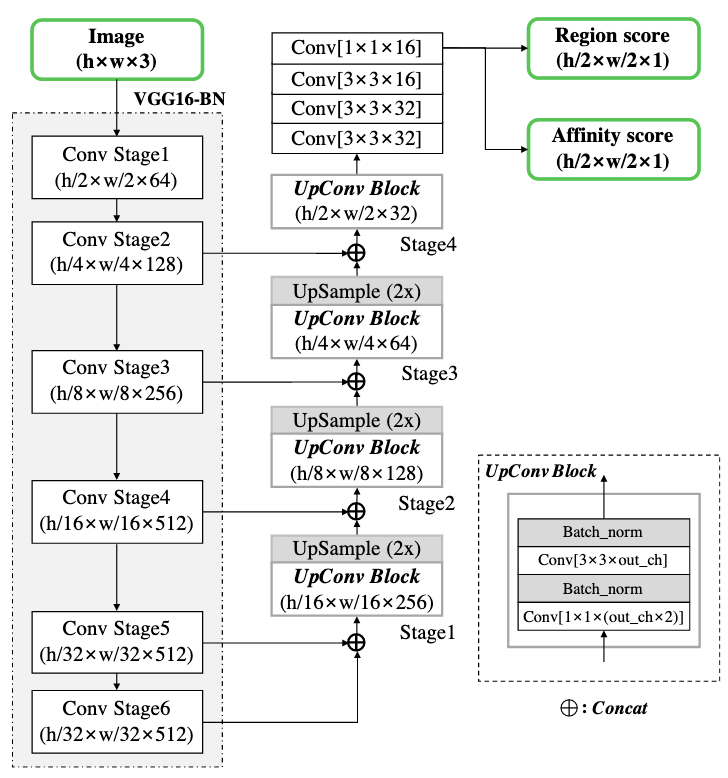
\includegraphics[width=0.5\textwidth]{img/craftstructure.png}
	\caption{Structure of Craft, adopted from~\protect\cite{CraftBaekEtAl}}
	\label{fig:craft1}
\end{figure}

As stated in the original paper, CRAFT adopts a fully convolutional network architecture based on VGG-16 \citep{vgg} with batch normalization as its backbone \citep{CraftBaekEtAl}.
It is further described as follow:
\begin{quotation}
	\emph{``Our model has skip connections in the decoding part, which is similar to U-Net \citep{unet} in that it aggregates low level features. The final output has two channels as score maps: the region score and the affinity score.
	The network architecture is schematically illustrated in figure~\ref{fig:craft1} \citep{CraftBaekEtAl}.''}
\end{quotation}
% subsection overviewcraft (end)
% section overviewmethods (end)

\section{Methodology} % (fold)
\label{sec:methodology}
asddssafs
% section methodology (end)

\section{Results and Evaluation} % (fold)
\label{sec:evaluation}
asdasdssada
% section evaluation (end)

\section{Conclusion} % (fold)
\label{sec:conclusion}
Lorem ipsum dolor sit amet, consetetur sadipscing elitr, sed diam nonumy eirmod tempor invidunt ut labore et dolore magna aliquyam erat, sed diam voluptua. At vero eos et accusam et justo duo dolores et ea rebum. Stet clita kasd gubergren, no sea takimata sanctus est Lorem ipsum dolor sit amet. Lorem ipsum dolor sit amet, consetetur sadipscing elitr, sed diam nonumy eirmod tempor invidunt ut labore et dolore magna aliquyam erat, sed diam voluptua. At vero eos et accusam et justo duo dolores et ea rebum. Stet clita kasd gubergren, no sea takimata sanctus est Lorem ipsum dolor sit amet.
% section conclusion (end)

\section{Section about quotations} % (fold)
\label{sec:section_about_quotations}

In this section, an example for a literal quotation is given. 

\begin{quotation}
	\emph{``A persona is a rich picture of an imaginary person who represents your core user group.''}
	\citep{CraftBaekEtAl}
\end{quotation}

Sometimes you might want to make use of the authors name within the text. Before, we used the command \texttt{citep\{\}}, which creates the brackets around author name and year. You can also use the \texttt{cite} command like this: \\

\cite{CraftBaekEtAl} defined the concept of persona as follows: 
\begin{quotation}
	\emph{``A persona is a rich picture of an imaginary person who represents your core user group.''}
	\citep{EastZhouEtAl}
\end{quotation}

You may notice, that this increases the readability of the text. \\

According to APA format\footnote{ American Psychological Association (APA)} there are some rules, when and how to include page numbers, when referring to literature. 

\begin{quotation}
	\emph{``Include page numbers for any citations in the text of your paper that include direct quotations or refer to a specific part of the work you are referencing. Direct quotations must include a page number as part of the citation. The quoted material should be followed by a citation in parentheses that gives the author's name, the year in which the work was published, and the page number from which the quoted material appears.''}
	\citep{LongEtAl}
\end{quotation}

Check out the example and recommendations of \cite{LongEtAl} on \url{http://www.ehow.com/how_5689799_cite-numbers-apa-format.html}. In \LaTeX you can include the pages very easy. For example: \\

 stated: 

\begin{quotation}
	\emph{``We hope that our preliminary attempts to begin answering the question will convince the reader, not necessarily that our views are correct, but that the question was and is well worth asking''}
	\citep{CraftBaekEtAl}
\end{quotation}

Note that in the first reference, we used \texttt{citet[]\{\}} in order to have brackets just around year and page number; later we used \texttt{citep[]\{\}}.

% section section_about_quotations (end)


\section{Section about references within the document} % (fold)
\label{sec:section_about_references_within_the_document}

If you want to refer to you own chapters, figures, tables or the like, you can make use of the \texttt{ref\{\}} command, for example:
\begin{itemize}
	\item section~\ref{sec:section_about_quotations} on page \pageref{sec:section_about_quotations}
\end{itemize} 



% section section_about_references_within_the_document (end)

\subsection{Subsection within Foundations} % (fold)
\label{sub:subsection_within_foundations}
Lorem ipsum dolor sit amet, consetetur \cite{NaturalScene} sadipscing elitr, sed diam nonumy eirmod tempor invidunt ut labore et dolore magna aliquyam erat, sed diam voluptua. At vero eos et accusam et justo duo dolores et ea rebum. Stet clita kasd gubergren, no sea takimata sanctus est Lorem ipsum dolor sit amet. Lorem ipsum dolor sit amet, consetetur sadipscing elitr, sed diam nonumy eirmod tempor invidunt ut labore et dolore magna aliquyam erat, sed diam voluptua. At vero eos et accusam et justo duo dolores et ea rebum. Stet clita kasd gubergren, no sea takimata sanctus est Lorem ipsum dolor sit amet.
% subsection subsection_within_foundations (end)

\subsection{Another subsection within Foundations} % (fold)
\label{sub:another_subsection_within_foundations}
Lorem ipsum dolor sit amet, consetetur sadipscing \cite{Rosebrockeast} elitr, sed diam nonumy eirmod tempor invidunt ut labore et dolore magna aliquyam erat, sed diam voluptua. At vero eos et accusam et justo duo dolores et ea rebum. Stet clita kasd gubergren, no sea takimata sanctus est Lorem ipsum dolor sit amet. Lorem ipsum dolor sit amet, consetetur sadipscing elitr, sed diam nonumy eirmod tempor invidunt ut labore et dolore magna aliquyam erat, sed diam voluptua. At vero eos et accusam et justo duo dolores et ea rebum. Stet clita kasd gubergren, no sea takimata sanctus est Lorem ipsum dolor sit amet.
% subsection another_subsection_within_foundations (end)


% section foundations (end)

\newpage 

\bibliographystyle{natdin}
	\bibliography{references} % expects file "references.bib"
	\addcontentsline{toc}{section}{References}
\end{document}